\chapter{连续函数空间}

\vspace{-2 em}
\section{有界连续函数}

设 $E$ 是一个度量空间.记 $\mathcal{C}\left( E\right)$ 为所有连续实值(可能无界)函数 $f : E \mapsto  \mathbb{R}$ 构成的空间.一般而言，该空间没有自然范数.因此，我们还将考虑所有有界连续函数 $f : E \mapsto  \mathbb{R}$ 构成的空间 $\mathcal{B}C\left( E\right)$ ，其范数为
\begin{equation}\tag{3.1}\label{eq:bc-norm}
\| f\|  \doteq  \mathop{\sup }\limits_{{x \in  E}}\left| {f\left( x\right) }\right| .
\end{equation}


本章大部分内容将讨论 $E$ 为紧集的情形.此时，每个连续函数 $f : E \mapsto  \mathbb{R}$ 必然有界，故 $\mathcal{C}\left( E\right)  = \mathcal{B}C\left( E\right)$ .

\begin{lemma}\label{lem:bc-banach}
$\mathcal{B}C\left( E\right)$ 是一个Banach空间.
\end{lemma}

\begin{proof}
1. 设 ${\left( {f}_{n}\right) }_{n \geq  1}$ 是 $\mathcal{B}C\left( E\right)$ 中的一个柯西列.则对每个固定的 $x \in  E$ ，数列 ${f}_{n}\left( x\right)$ 是柯西列，因而收敛于某个极限，记为 $f\left( x\right)$ .

2. 由假设，对每个 $\varepsilon  > 0$ ，存在足够大的 $N$ ，使得
\[
\mathop{\sup }\limits_{{x \in  E}}\left| {{f}_{n}\left( x\right)  - {f}_{m}\left( x\right) }\right|  \leq  \varepsilon \;\forall\,n,m \geq  N.
\]

令 $m \rightarrow  \infty$ ，由于 ${f}_{m}\left( x\right)  \rightarrow  f\left( x\right)$ ，得
\[
\mathop{\sup }\limits_{{n \geq  N}}\mathop{\sup }\limits_{{x \in  E}}\left| {{f}_{n}\left( x\right)  - f\left( x\right) }\right|  \leq  \varepsilon .
\]

进而可得
\[
\mathop{\sup }\limits_{{n \geq  N}}\norm{{f}_{n} - f} \leq  \varepsilon ,\;\mathop{\sup }\limits_{{x \in  E}}\left| {f\left( x\right) }\right|  \leq  \varepsilon  + \mathop{\sup }\limits_{{x \in  E}}\left| {{f}_{N}\left( x\right) }\right|  < \infty .
\]
由于$\varepsilon$是任意的，第一个不等式表明 $\norm{{f}_{n} - f} \rightarrow  0$ 收敛；第二个不等式表明 $f$ 有界.

3. 最后，我们证明 $f$ 连续.任给 $x \in  E$ 和 $\varepsilon  > 0$ .由一致收敛性，存在整数 $N$ ，使得对所有 $x \in  E$ 均有 $\left| {{f}_{N}\left( x\right)  - f\left( x\right) }\right|  < \varepsilon /3$ .又因 ${f}_{N}$ 连续，故存在 $\delta  > 0$ ，使得当 $d\left( {y,x}\right)  < \delta$ 时有 $\left| {{f}_{N}\left( y\right)  - {f}_{N}\left( x\right) }\right|  < \varepsilon /3$ .综合上述不等式，当 $d\left( {y,x}\right)  < \delta$ 时，有
{\setjot[-2]\begin{align*}
\left| {f\left( y\right)  - f\left( x\right) }\right|  &\leq  \left| {f\left( y\right)  - {f}_{N}\left( y\right) }\right|  + \left| {{f}_{N}\left( y\right)  - {f}_{N}\left( x\right) }\right|  + \left| {{f}_{N}\left( x\right)  - f\left( x\right) }\right|\\
&< \frac{\varepsilon }{3} + \frac{\varepsilon }{3} + \frac{\varepsilon }{3} = \varepsilon
\end{align*}}

从而证得 $f$ 在点 $x$ 处连续.
\end{proof}

\begin{note}[逐点收敛与一致收敛]\label{rem:pointwise-vs-uniform}
前面的论证表明，如果连续函数序列 ${f}_{n}$一致收敛于函数 $f$ ，那么 $f$ 也是连续的.另一方面，连续函数序列可以逐点收敛到一个不连续的极限.例如，在区间 $E = \left(  {0,1}\right)$ 上，函数序列 ${f}_{n}\left( x\right)  = {x}^{n}$ 逐点收敛到不连续函数
\[
f\left( x\right)  =
\begin{cases}
0, & 0 \leq x < 1,\\
1, & x = 1.
\end{cases}
\]

显然，此处的收敛在整区间 $\left(  {0,1}\right)$ 上并非一致收敛.
\end{note}

以下定理描述了一种逐点收敛蕴含一致收敛的情形.我们回顾:函数列 ${f}_{n} : E \mapsto  \mathbb{R}$ 称为递增的，若 $m < n$ 蕴含 ${f}_{m}\left( x\right)  \leq  {f}_{n}\left( x\right)$ 对所有 $x \in  E$ 成立.

\begin{theorem}[Dini]\label{thm:dini}
设 $E$ 为紧致度量空间.若 ${\left( {f}_{n}\right) }_{n \geq  1}$ 是 $\mathcal{C}\left( E\right)$ 中一列递增函数，且逐点收敛于连续极限函数 $f$ ，则 ${f}_{n} \rightarrow  f$ 在 $E$ 上一致收敛.
\end{theorem}

\begin{proof}
任取$\varepsilon  > 0$，由假设，对每个$x \in  E$，存在整数$N\left( x\right)$，使得$\left| {{f}_{N\left( x\right) }\left( x\right)- f\left( x\right) }\right|  < \varepsilon$.

由于 ${f}_{N\left( x\right) }$ 与 $f$ 连续，存在 $x$ 的一个开邻域 ${V}_{x}$ ，使得对每个 $y \in  {V}_{x}$ ，均有 $\left| {{f}_{N\left( x\right) }\left( y\right)  - {f}_{N\left( x\right) }\left( x\right) }\right|  < \varepsilon$ 且 $\left| {f\left( y\right)  - f\left( x\right) }\right|  < \varepsilon$ .

由于 $E$ 紧致，可用其中有限个此类邻域覆盖 $E$ ，记为 $E \subseteq  {V}_{{x}_{1}} \cup  \cdots  \cup  {V}_{{x}_{m}}$ .

取整数 $N = \max \left\{  {N\left( {x}_{1}\right) ,\ldots ,N\left( {x}_{m}\right) }\right\}$ .\par
对任意 $n \geq  N$ 与 $y \in  E$ ，若假设 $y \in  {V}_{{x}_{i}}$，则有
\[
{f}_{N\left( {x}_{i}\right) }\left( y\right)  \leq  {f}_{N}\left( y\right)  \leq  {f}_{n}\left( y\right)  \leq  f\left( y\right) ,
\]

因为该序列递增.故
{\setjot[-2]\begin{align*}
\left| {{f}_{n}\left( y\right)  - f\left( y\right) }\right|  &\leq  \left| {{f}_{N\left( {x}_{i}\right) }\left( y\right)  - f\left( y\right) }\right| \\
&\leq  \left| {{f}_{N\left( {x}_{i}\right) }\left( y\right)  - {f}_{N\left( {x}_{i}\right) }\left( {x}_{i}\right) }\right|  + \left| {{f}_{N\left( {x}_{i}\right) }\left( {x}_{i}\right)  - f\left( {x}_{i}\right) }\right|  + \left| {f\left( {x}_{i}\right)  - f\left( y\right) }\right| \\
&< \varepsilon  + \varepsilon  + \varepsilon=3\varepsilon.
\end{align*}}


由于 $y \in  E$ 与 $\varepsilon  > 0$ 是任意的，这就确立了 ${f}_{n} \rightarrow  f$ 的一致收敛性.
\end{proof}

\section{Stone-Weierstrass逼近定理}

给定定义域 $E \subset  {\mathbb{R}}^{n}$ ，在计算中，用特殊函数(如多项式、指数函数或三角多项式)逼近连续实值函数 $f \in  \mathcal{B}C\left( E\right)$ 可能很有用.因此，理解是否每个函数 $f \in  \mathcal{B}C\left( E\right)$ 均可被此类函数一致逼近至关重要.本节将证明该方向的一个关键结果.

作为预备知识，注意到空间 $\mathcal{B}C\left( E\right)$ 构成一个代数:即它对乘法封闭:
\[
\text{若}\,f,g \in  \mathcal{B}C\left( E\right),\,\text{那么}\,{fg} \in  \mathcal{B}C\left( E\right) \text{ . }
\]

此外，乘积的范数满足
\[
\| {fg}\|  \leq  \| f\| \| g\| .
\]

我们称子空间 $\mathcal{A} \subseteq  \mathcal{B}C\left( E\right)$ 为子代数，若 $f,g \in  \mathcal{A}$ 蕴含 ${fg} \in  \mathcal{A}$ .

\begin{lemma}[子代数的闭包]\label{lem:subalgebra-closure}
若 $\mathcal{A} \subseteq  \mathcal{B}C\left( E\right)$ 是子代数，则其闭包 $\overline{\mathcal{A}}$ 也是子代数.
\end{lemma}

\begin{proof}
事实上，设 $f,g \in  \overline{\mathcal{A}}$ .则存在一致收敛序列 ${f}_{n},{g}_{n} \in  \mathcal{A}$ ，满足 ${f}_{n} \rightarrow  f$ 且 ${g}_{n} \rightarrow  g$.于是有
\[
\norm{{fg} - {f}_{n}{g}_{n}}\; \leq  \;\norm{{fg} - {f}_{n}g} + \norm{{f}_{n}g - {f}_{n}{g}_{n}}\; \leq  \;\norm{f - {f}_{n}}\norm{g} + \norm{f}_{n}\norm{g - {g}_{n}}.
\]

由于序列 ${\left( {f}_{n}\right) }_{n \geq  1}$ 一致有界，当 $n \rightarrow  \infty$ 时，右端趋近于零.这表明 ${f}_{n}{g}_{n} \rightarrow  {fg}$ 收敛.又因 $\mathcal{A}$ 是一个代数，故对每个 $n$ 均有 ${f}_{n}{g}_{n} \in  \mathcal{A}$ .因此 ${fg} \in  \overline{\mathcal{A}}$ .
\end{proof}

我们称子集 $\mathcal{A} \subseteq  \mathcal{B}C\left( E\right)$ 分离点，若对任意两个不同点 $x,y \in  E$ ，存在函数 $f \in  \mathcal{A}$ 使得 $f\left( x\right)  \neq \; f\left( y\right)$ .

\begin{theorem}[Stone-Weierstrass]\label{thm:stone-weierstrass}
设 $E$ 为紧致度量空间.若 $\mathcal{A}$ 是 $\mathcal{C}\left( E\right)$ 的一个分离点且包含常值函数的子代数，则 $\overline{\mathcal{A}} = \mathcal{C}\left( E\right)$ .

换言之，设 $\mathcal{A}$ 是一族定义在 $f : E \mapsto  \mathbb{R}$ 上的连续实值函数，满足如下性质:

(i) 若 $f,g \in  \mathcal{A}$ 且 $a,b \in  \mathbb{R}$ ，则线性组合 ${af} + {bg}$ 属于 $\mathcal{A}$ .

(ii) 若 $f,g \in  \mathcal{A}$ ，则乘积 ${fg}$ 也属于 $\mathcal{A}$ .

(iii) 常值函数 $f\left( x\right)  \equiv  1$ 属于 $\mathcal{A}$ .

(iv) 对任意两个不同点 $x,y \in  E$ ，存在 $f \in  \mathcal{A}$ 使得 $f\left( x\right)  \neq  f\left( y\right) .$ .

则定义在紧致区域 $E$ 上的每个连续函数 $f : E \mapsto  \mathbb{R}$ 均可由 $\mathcal{A}$ 中的函数一致逼近.
\end{theorem}

\begin{proof}
1. 存在一列多项式 ${\left( {p}_{n}\right) }_{n \geq  1}$ ，使得 ${p}_{n}\left( t\right)  \rightarrow \; \sqrt{t}$ 在 $t \in  \left(  {0,1}\right)$ 上一致成立.

为证上述断言，其基本思想是通过迭代构造方程 $t - {p}^{2}\left( t\right)  = 0$ 的近似解.于是令 ${p}_{0}\left( t\right)  \equiv  0$ ，并依 $n = 0,1,2,\ldots$ 归纳地定义:
\begin{equation}\tag{3.2}\label{eq:pn-iteration}
{p}_{n + 1}\left( t\right)  = {p}_{n}\left( t\right)  + \frac{1}{2}\left( {t - {p}_{n}^{2}\left( t\right) }\right)
\end{equation}
(见图\ref{fig:pn-polynomials}).由归纳法可验证：对每个 $t \in  \left(  {0,1}\right)$ ，均有 ${p}_{n}\left( t\right)  \leq  {p}_{n + 1}\left( t\right)  \leq  \sqrt{t}$ .事实上，
\begin{align*}
\sqrt{t} - {p}_{n + 1}\left( t\right)  &= \sqrt{t} - {p}_{n}\left( t\right)  - \frac{1}{2}\left( {t - {p}_{n}^{2}\left( t\right) }\right)\\
&= \left( {\sqrt{t} - {p}_{n}\left( t\right) }\right) \left( {1 - \frac{1}{2}\left( {\sqrt{t} + {p}_{n}\left( t\right) }\right) }\right)  \geq  0.
\end{align*}


对每个固定的 $t \in  \left(  {0,1}\right)$ ，序列 ${p}_{n}\left( t\right)$ 单调递增且上有界，故存在唯一极限，记为 $g\left( t\right)$ .由 \eqref{eq:pn-iteration} 知该极限满足 $t - {g}^{2}\left( t\right)  = 0$ .又因 $g\left( t\right)  \geq  0$ ，故得 $g\left( t\right)  = \sqrt{t}$ .

最后，由定理\ref{thm:dini}可知，该收敛在 $t \in  \left(  {0,1}\right)$ 上是一致的.

\begin{figure}[htbp]
\centering
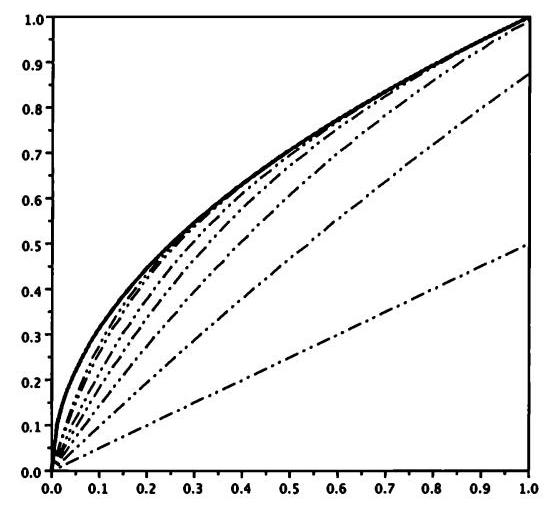
\includegraphics[width=0.4\textwidth]{images/bo_d6ik6nn7aajc739ct1l0_61_464_229_545_507_0.jpg}
\captionof{figure}{由式\eqref{eq:pn-iteration}定义的序列中的前几个多项式.}
\label{fig:pn-polynomials}
\end{figure}

\noindent 2. 对任意函数 $f \in  \mathcal{A}$ ，均有 $\left| f\right|  \in  \overline{\mathcal{A}}$ .

事实上，令 $\kappa  \doteq  \mathop{\max }\limits_{{x \in  E}}\left| {f\left( x\right) }\right|$ .可设 $\kappa  \neq  0$ .于是所有函数 ${f}_{n}\left( x\right)  = {p}_{n}\left( {{f}^{2}\left( x\right) /{\kappa }^{2}}\right)$ 均属于 $\mathcal{A}$ ，因为 $\mathcal{A}$ 是一个代数.又因 ${f}^{2}\left( x\right) /{\kappa }^{2} \in \; \left(  {0,1}\right)$ ，上一步推出收敛
\[
{f}_{n}\left( x\right)  \rightarrow  \sqrt{\frac{{f}^{2}\left( x\right) }{{\kappa }^{2}}} = \frac{\left| f\left( x\right) \right| }{\kappa },
\]

在 $x \in  E$ 上一致成立.因此 $\frac{\left| f\right| }{\kappa } \in  \overline{\mathcal{A}}$ ，从而 $\left| f\right|  \in  \overline{\mathcal{A}}$ 亦然.

\noindent 3. 现将前述论证应用于子代数 $\overline{\mathcal{A}}$ ，可得:若 $f,g \in  \overline{\mathcal{A}}$ ，则函数
\[
\max \{ f,g\}  = \frac{1}{2}\left( {f + g + \left| {f - g}\right| }\right) ,\;\min \{ f,g\}  = \frac{1}{2}\left( {f + g - \left| {f - g}\right| }\right)
\]
也属于 $\overline{\mathcal{A}}$ .

\noindent 4. 对任意两个不同点 ${y}_{1},{y}_{2} \in  E$ 及任意一对实数 ${a}_{1},{a}_{2}$ ，存在一函数 $f \in  \mathcal{A}$ ，使得 $f\left( {y}_{1}\right)  = {a}_{1}$ 且 $f\left( {y}_{2}\right)  = {a}_{2}$ .

事实上，由假设，存在一连续函数 $g \in  \mathcal{A}$ ，使得 $g\left( {y}_{1}\right)  \neq  g\left( {y}_{2}\right)$ .由于 $\mathcal{A}$ 是一个代数且包含所有常值函数，故函数
\[
f\left( x\right)  \doteq  {a}_{1} + \left( {{a}_{2} - {a}_{1}}\right) \frac{g\left( x\right)  - g\left( {y}_{1}\right) }{g\left( {y}_{2}\right)  - g\left( {y}_{1}\right) }
\]
属于 $\mathcal{A}$ ，并满足我们的要求.

\noindent 5. 对任意连续函数 $f$ 、一点 $y \in  E$ 及 $\varepsilon  > 0$ ，存在一函数 ${g}_{y} \in  \overline{\mathcal{A}}$ ，使得
\begin{equation}\tag{3.3}\label{eq:gy-ineq}
{g}_{y}\left( y\right)  = f\left( y\right) ,\;{g}_{y}\left( x\right)  \leq  f\left( x\right)  + \varepsilon ,\;\forall\,x \in  E.
\end{equation}

\begin{figure}[htbp]
    \vspace{-1 em}
\centering
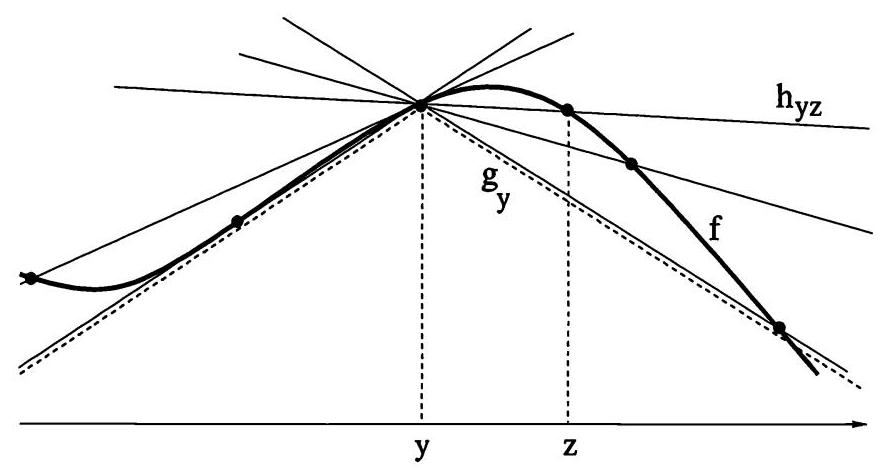
\includegraphics[width=0.7\textwidth]{images/bo_d6ik6nn7aajc739ct1l0_62_300_227_883_472_0.jpg}
\captionof{figure}{对固定 $y$ ，取有限个函数 ${h}_{yz}$ (此处绘为仿射函数)的下确界，得到一连续函数 ${g}_{y} \leq  f + \varepsilon$ ，且满足 ${g}_{y}\left( y\right)  = f\left( y\right)$ .}
\label{fig:gy-min}
\end{figure}

事实上(见图\ref{fig:gy-min})，由上一步可知，对每一点 $z \in  E$ ，存在一函数 ${h}_{yz} \in  \mathcal{A}$ ，使得 ${h}_{yz}\left( y\right)  = f\left( y\right)$ 且 ${h}_{yz}\left( z\right)  = f\left( z\right)$ .

由于 $f$ 与 ${h}_{yz}$ 均连续，故存在 $z$ 的一个开邻域 ${V}_{z}$ ，使得对每个 $x \in  {V}_{z}$ 均有 ${h}_{yz}\left( x\right)  < f\left( x\right)  + \varepsilon$ .

我们可用有限个此类邻域覆盖紧集 $E$ : $E \subseteq  {V}_{{z}_{1}} \cup  \cdots  \cup  {V}_{{z}_{m}}$ .于是函数
\[
{g}_{y}\left( x\right)  \doteq  \min \left\{  {{h}_{y{z}_{1}}\left( x\right) ,\ldots ,{h}_{y{z}_{m}}\left( x\right) }\right\}
\]

位于 $\overline{\mathcal{A}}$ 中，且满足\eqref{eq:gy-ineq}中的条件.

\begin{figure}[H]
    \vspace{-1 em}
\centering
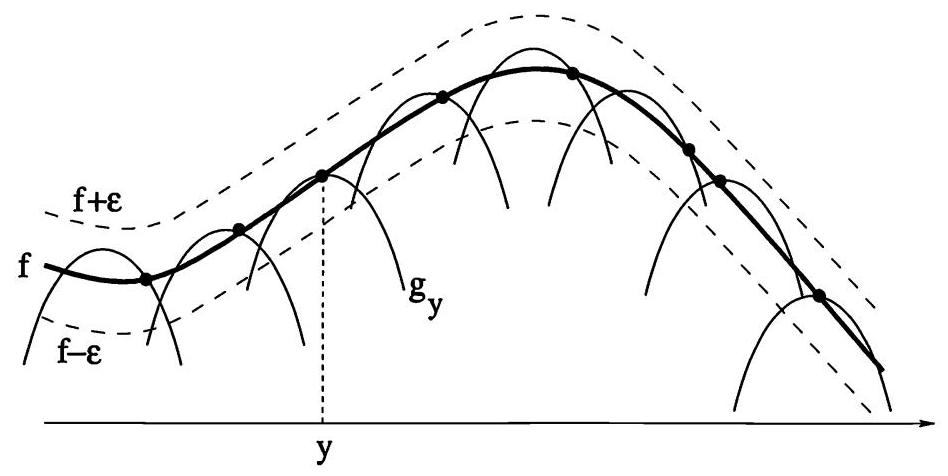
\includegraphics[width=0.7\textwidth]{images/bo_d6ik6nn7aajc739ct1l0_62_266_1404_948_476_0.jpg}
\captionof{figure}{对有限个函数 ${g}_{y}$ 取上确界，得到一个连续函数 $g$ ，使得 $f - \varepsilon  \leq  g \leq  f + \varepsilon$ .}
\label{fig:g-max}
\end{figure}

\noindent 6. $\mathcal{A}$ 的闭包是整个空间 $\mathcal{C}\left( E\right)$ .

事实上，设 $f \in  \mathcal{C}\left( E\right)$ 为任意连续函数， $\varepsilon  > 0$ 给定.对每个 $y \in  E$ ，由前一步可知存在函数 ${g}_{y} \in  \overline{\mathcal{A}}$ (见图\ref{fig:g-max})，使得
\[
{g}_{y}\left( y\right)  = f\left( y\right) ,\;{g}_{y}\left( x\right)  \leq  f\left( x\right)  + \varepsilon ,\;\forall\,x \in  E.
\]

由 $f$ 与 ${g}_{y}$ 的连续性，存在 $y$ 的一个邻域 ${U}_{y}$ ，使得
\[
{g}_{y}\left( x\right)  \geq  f\left( x\right)  - \varepsilon \;\forall\,x \in  {U}_{y}.
\]

现用有限个邻域 $E \subseteq \; {U}_{{y}_{1}} \cup  \cdots  \cup  {U}_{{y}_{\nu }}$ 覆盖紧集 $E$ .则函数
\[
g\left( x\right)  \doteq  \max \left\{  {{g}_{{y}_{1}}\left( x\right) ,\ldots ,{g}_{{y}_{\nu }}\left( x\right) }\right\}
\]

位于 $\overline{\mathcal{A}}$ 中，且满足
\[
f\left( x\right)  - \varepsilon  \leq  g\left( x\right)  \leq  f\left( x\right)  + \varepsilon \;\forall\,x \in  E.
\]

\end{proof}

满足定理\ref{thm:stone-weierstrass}全部假设的一个自然代数例子是多项式函数.

\begin{corollary}[多项式一致逼近]\label{cor:poly-approx}
设 $E$ 为 ${\mathbb{R}}^{n}$ 的紧子集， $\mathcal{A}$ 为变量 $\left( {{x}_{1},\ldots ,{x}_{n}}\right)$ 的所有实值多项式构成的族，则 $\mathcal{A}$ 在 $\mathcal{C}\left( E\right)$ 中稠密.
\end{corollary}

\begin{proof}
事实上， $\left( {{x}_{1},\ldots ,{x}_{n}}\right)$ 上的所有实值多项式构成的族是一个代数，它包含常值函数且能分离 ${\mathbb{R}}^{n}$ 中的点.因此，由定理\ref{thm:stone-weierstrass}，每个连续函数 $f : E \mapsto  \mathbb{R}$ 均可被多项式一致逼近.
\end{proof}

\subsection{复值函数}

定理\ref{thm:stone-weierstrass}证明中的一个关键要素是:若两个实值函数 $f,g$ 属于某个子代数 $\mathcal{A}$ ，则 $\max \{ f,g\}$ 与 $\min \{ f,g\}$ 也属于 $\overline{\mathcal{A}}$ .显然，此类陈述对复值函数毫无意义.事实上，Stone-Weierstrass定理在其原始形式下对复值函数并不成立.

为获得适用于函数 $f : E \mapsto  \mathbb{C}$ 的逼近结果，主要思路是将 $\mathbb{C} = \mathbb{R} \oplus  i\mathbb{R}$ 视为实数域上的二维空间.以下，对任意紧度量空间 $E$ ，我们用 ${\mathcal{C}}_{\mathbb{R}}\left( {E;\mathbb{C}}\right)$ 表示 $E$ 上所有连续复值函数构成的空间，并将其视作实数域上的向量空间.

\begin{theorem}\label{thm:stone-weierstrass-complex}
设 $E$ 为紧度量空间， $\mathcal{A}$ 为 ${\mathcal{C}}_{\mathbb{R}}\left( {E;\mathbb{C}}\right)$ 的一个子代数，它能分离点并包含常值函数；此外，若 $f \in  \mathcal{A}$ ，则其复共轭函数 $\bar{f}$ 亦属于 $\mathcal{A}$ .则 $\mathcal{A}$ 在 ${\mathcal{C}}_{\mathbb{R}}\left( {E;\mathbb{C}}\right)$ 中稠密.
\end{theorem}

\begin{proof}
1. 根据假设，若 $f \in  \mathcal{A}$ ，则其实部与虚部
\[
\operatorname{Re}\left( f\right)  = \frac{f + \bar{f}}{2},\;\operatorname{Im}\left( f\right)  = \frac{f - \bar{f}}{2}
\]
同样位于 $\mathcal{A}$ 中.设 ${\mathcal{A}}_{0}$ 为 $\mathcal{A}$ (在实数域上)的子代数，由所有取实数值的函数 $f \in  \mathcal{A}$ 构成.对 ${\mathcal{A}}_{0}$ 应用定理\ref{thm:stone-weierstrass}，可得 ${\mathcal{A}}_{0}$ 在 $\mathcal{C}\left( E\right)  = {\mathcal{C}}_{\mathbb{R}}\left( {E;\mathbb{R}}\right)$ 中稠密.

\noindent 2. 给定任意 $f \in  {\mathcal{C}}_{\mathbb{R}}\left( {E;\mathbb{C}}\right)$ ，我们将 $f$ 写为其实部与虚部之和 $f = \operatorname{Re}\left( f\right)  + i\operatorname{Im}\left( f\right)$ .由前一步可知，存在两个实值函数序列 ${g}_{n},{h}_{n} \in  {\mathcal{A}}_{0}$ ，使得
\begin{equation}\tag{3.4}\label{eq:gh-conv}
{g}_{n} \rightarrow  \operatorname{Re}\left( f\right) ,\;{h}_{n} \rightarrow  \operatorname{Im}\left( f\right)
\end{equation}

作为 $n \rightarrow  \infty$ ，在 $E$ 上一致地.

考虑序列 ${f}_{n} \doteq  {g}_{n} + i{h}_{n} \in  {\mathcal{A}}_{0} + i{\mathcal{A}}_{0} = \mathcal{A}$ .由\eqref{eq:gh-conv}式，我们有一致收敛性 ${f}_{n} \rightarrow  f$.因此 $\overline{\mathcal{A}} = {\mathcal{C}}_{\mathbb{R}}\left( {E;\mathbb{C}}\right)$ .
\end{proof}

\begin{instance}[复三角多项式]\label{ins:complex-trig-poly}
设 $E$ 为 ${\mathbb{R}}^{2}$ 中的单位圆周 $\left\{  {{x}^{2} + {y}^{2} = 1}\right\}$ . $E$ 上的点将由角度 $\theta  \in  \left(  {0,{2\pi }}\right)$ 参数化.令 $\mathcal{A}$ 为所有复三角多项式构成的代数:
\begin{equation}\tag{3.5}\label{eq:complex-trig}
p\left( \theta \right)  = \mathop{\sum }\limits_{{n =  - N}}^{N}{\mathrm{c}}_{n}{e}^{in\theta }
\end{equation}

其中 $N \geq  0$ 为任意整数，系数 ${\mathrm{c}}_{n}$ 为复数.显然， $\mathcal{A}$ 是一个代数，包含常值函数，且能分离点.此外， $p \in  \mathcal{A}$ 也蕴含 $\bar{p} \in  \mathcal{A}$ .由定理\ref{thm:stone-weierstrass-complex} 可知，所有这类复三角多项式构成的族在 ${\mathcal{C}}_{\mathbb{R}}\left( {E;\mathbb{C}}\right)$ 中稠密.
\end{instance}

沿用例\ref{ins:complex-trig-poly}，我们现在证明:一个实值的连续周期函数可用如下形式的三角多项式一致逼近
\begin{equation}\tag{3.6}\label{eq:real-trig}
q\left( x\right)  = \mathop{\sum }\limits_{{k = 0}}^{N}{\alpha }_{k}\cos {kx} + \mathop{\sum }\limits_{{k = 1}}^{N}{\beta }_{k}\sin {kx}.
\end{equation}

此处 $N \geq  1$ 为任意整数，而 ${\alpha }_{n},{\beta }_{n}$ 为实数.

\begin{corollary}[三角多项式对周期函数的逼近]\label{cor:trig-approx-periodic}
设 $f : \mathbb{R} \mapsto  \mathbb{R}$ 是一个连续函数，且以 ${2\pi }$ 为周期.则对任意 $\varepsilon  > 0$ ，存在形如 \eqref{eq:real-trig} 的三角多项式 $q$ ，使得
\begin{equation}\tag{3.7}\label{eq:trig-approx-bound}
\left| {q\left( x\right)  - f\left( x\right) }\right|  \leq  \varepsilon ,\;\forall\,x \in  \mathbb{R}.
\end{equation}
\end{corollary}

\begin{proof}
由假设，对每个 $x \in  \mathbb{R}$ ，均有 $f\left( {x + {2\pi }}\right)  = f\left( x\right)$ .如例\ref{ins:complex-trig-poly}所示，存在一个形如\eqref{eq:complex-trig}的复三角多项式 $p$ ，使得
\begin{equation}\tag{3.8}\label{eq:complex-approx-bound}
\left| {p\left( x\right)  - f\left( x\right) }\right|  \leq  \varepsilon \;\forall\,x \in  \mathbb{R}.
\end{equation}

考虑复系数 ${c}_{n} = {a}_{n} + i{b}_{n}$ ，其中 ${a}_{n},{b}_{n} \in  \mathbb{R}$ .记 $q\left( x\right)  \doteq  \operatorname{Re}p\left( x\right)$ 为 $p$ 的实部，我们计算
\[
q\left( x\right)  = \mathop{\sum }\limits_{{n =  - N}}^{N}{a}_{n}\cos {nx} - \mathop{\sum }\limits_{{n =  - N}}^{N}{b}_{n}\sin {nx} = \mathop{\sum }\limits_{{n = 0}}^{N}{\alpha }_{n}\cos {nx} + \mathop{\sum }\limits_{{n = 1}}^{N}{\beta }_{n}\sin {nx},
\]

其中${\alpha }_{0} = {a}_{0},\;{\alpha }_{n} = {a}_{-n} + {a}_{n},\;{\beta }_{n} = {b}_{-n} - {b}_{n}\,\text{若}\,n \geq  1.$

由于 $f$ 是实值函数，由\eqref{eq:complex-approx-bound}式可得
{\setjot[-2]\begin{align*}
\left| {q\left( x\right)  - f\left( x\right) }\right|  &= \left| {\operatorname{Re}p\left( x\right)  - \operatorname{Re}f\left( x\right) }\right| \\
&\leq  \left| {p\left( x\right)  - f\left( x\right) }\right|  \leq  \varepsilon \;,\forall\,x \in  \mathbb{R}.\qedhere
\end{align*}}
\end{proof}

\begin{remark}\label{rem:even-odd-trig}
若周期函数 $f$ 是偶函数，即满足 $f\left( x\right)  = f\left( {-x}\right)$ ，则它可用形如\eqref{eq:real-trig}的三角多项式逼近，且对每个 $k \geq  1$ 均有 ${\beta }_{k} = 0$ ，即仅含有限个余弦函数的和.

若 $f$ 是奇函数，即满足 $f\left( x\right)  =  - f\left( {-x}\right)$ ，则在\eqref{eq:real-trig}式中可取对每个 $k \geq  0$ 均有 ${\alpha }_{k} = 0$ .换言之， $f$ 可由有限个正弦函数的和逼近.
\end{remark}

\section{Ascoli紧性定理}

在有限维空间中，根据波尔查诺-Weierstrass定理，每个有界序列都存在收敛子列.另一方面，如第 2 章定理 2.22 所示，该紧性性质在任意无限维赋范空间中均不成立.例如，在空间 $\mathcal{C}\left( \left(  {0,1}\right)  \right)$ 中，连续函数序列 ${f}_{n}\left( x\right)  = {x}^{n}$ 或 ${f}_{n}\left( x\right)  = \sin {nx}$ 虽有界，却不含一致收敛子列.因此自然提出问题:函数族 ${f}_{n}$ 需具备何种附加性质，才能保证存在一致收敛子列？Ascoli定理借助等度连续概念给出了一个回答.
\begin{definition}[等度连续]
    设 $E$ 为一度量空间.一族连续函数 $\mathcal{F} \subset  \mathcal{C}\left( E\right)$ 称为\colorbf{等度连续的}，若对任意 $x \in  E$ 和 $\varepsilon  > 0$ ，存在 $\delta  > 0$ ，使得对所有函数 $f \in  \mathcal{F}$，都有
\begin{equation}\tag{3.9}\label{eq:equicontinuity-point}
d\left( {y,x}\right)  < \delta \implies \left| {f\left( y\right)  - f\left( x\right) }\right|  < \varepsilon
\end{equation}
\end{definition}
注意此处 $\delta  > 0$ 可依赖于 $x$ 和 $\varepsilon$ ，但不依赖于特定函数 $f \in  \mathcal{F}$ .

\begin{lemma}\label{lem:equicontinuous-uniform}
设 $E$ 为紧致度量空间， $\mathcal{F} \subset  \mathcal{C}\left( E\right)$ 为等度连续族，则 $\mathcal{F}$ 是一致等度连续的.即对任意 $\varepsilon  > 0$ ，存在 $\delta  > 0$ ，使得
\begin{equation}\tag{3.10}\label{eq:equicontinuity-uniform}
d\left( {x,y}\right)  < \delta \implies \left| {f\left( x\right)  - f\left( y\right) }\right|  < \varepsilon ,\;\forall\,x,y \in  E,\;f \in  \mathcal{F}.
\end{equation}
\end{lemma}

\begin{proof}
给定 $\varepsilon  > 0$ .对每个 $x \in  E$ ，选取 $\delta  = \delta \left( x\right)  > 0$ ，使得\eqref{eq:equicontinuity-point}式对所有函数 $f \in  \mathcal{F}$ 同时成立.由紧性，可用有限个球覆盖空间 $E$ :
\[
E \subseteq  B\left( {{x}_{1},{\delta }_{1}}\right)  \cup  \cdots  \cup  B\left( {{x}_{n},{\delta }_{n}}\right) ,
\]
其中 ${\delta }_{i} = \delta \left( {x}_{i}\right)$ .选取足够小的 $\rho  > 0$ ，使得对每个 $x \in  E$ ，球 $B\left( {x,\rho }\right)$ 完全包含于某个球 $B\left( {{x}_{i},{\delta }_{i}}\right)$ 内.

现在假设 $d\left( {x,y}\right)  < \rho$ .则存在$k \in  \{ 1,\ldots ,n\}$ ，使得 $x,y \in  B\left( {{x}_{k},{\delta }_{k}}\right)$ .这意味着
\[
\left| {f\left( x\right)  - f\left( y\right) }\right|  \leq  \left| {f\left( x\right)  - f\left( {x}_{k}\right) }\right|  + \left| {f\left( y\right)  - f\left( {x}_{k}\right) }\right|  \leq  \varepsilon  + \varepsilon
\]
对每个函数 $f \in  \mathcal{F}$ 均成立.由于 $\varepsilon  > 0$ 是任意的，故该引理得证.
\end{proof}

若 $E$ 是紧度量空间，则 $\mathcal{C}\left( E\right)  = \mathcal{B}C\left( E\right)$ 是Banach空间.由完备性可知，对子集 $\mathcal{F} \subset  \mathcal{C}\left( E\right)$ ，以下性质等价:

(i) $\mathcal{F}$ 是相对紧的，即闭包 $\overline{\mathcal{F}}$ 是紧集.

(ii) $\mathcal{F}$ 是预紧的，即对任意 $\varepsilon  > 0$ ，它可被有限个半径为 $\varepsilon$ 的球覆盖.

(iii) 对任意连续函数序列 ${f}_{k} \in  \mathcal{F}$ ，均可提取一个子列，该子列在 $E$ 上一致收敛于某个函数 $f$ .

\begin{theorem}[Ascoli 定理]\label{thm:ascoli}
设 $E$ 是一个紧度量空间， $\mathcal{F} \subset  \mathcal{C}\left( E\right)$ 是一族等度连续函数，且满足
\begin{equation}\tag{3.11}\label{eq:ascoli-pointwise-bounded}
    \sup_{{f \in  \mathcal{F}}}\left| {f\left( x\right) }\right|  < \infty, \;\forall\,x \in  E.
\end{equation}

则 $\mathcal{F}$ 是 $\mathcal{C}\left( E\right)$ 中的相对紧子集.
\end{theorem}

\begin{proof}
只需证 $\mathcal{F}$ 是预紧的.

\noindent 1. 给定 $\varepsilon  > 0$ .由引理\ref{lem:equicontinuous-uniform}，存在 $\delta  > 0$ 使得\eqref{eq:equicontinuity-uniform}成立.由于 $E$ 是紧集，它可被有限个半径为$\delta$ 的球覆盖，记为
\[
E \subseteq  \mathop{\bigcup }\limits_{{i = 1}}^{n}B\left( {{x}_{i},\delta }\right) .
\]

由假设\eqref{eq:ascoli-pointwise-bounded}，
\[
M \doteq  \mathop{\max }\limits_{{i \in  \{ 1,\ldots ,n\} }}\mathop{\sup }\limits_{{f \in  \mathcal{F}}}\left| {f\left( {x}_{i}\right) }\right|  < \infty .
\]

现选取有限个数 ${\alpha }_{1},\ldots ,{\alpha }_{m}$ ，使得球 $B\left( {{\alpha }_{j},\varepsilon }\right)$ 覆盖紧区间 $\left(  {-M,M}\right)$ .

\noindent 2. 考虑所有映射 $\theta  : \left\{  {{x}_{1},\ldots ,{x}_{n}}\right\}   \mapsto  \left\{  {{\alpha }_{1},\ldots ,{\alpha }_{m}}\right\}$ 构成的集合 $\Theta$ .这是一个有限集；事实上，恰有 ${m}^{n}$ 个这样的映射.对每个 $\theta  \in  \Theta$ ，定义连续函数族
\[
{\mathcal{F}}_{\theta } \doteq  \left\{  {f \in  \mathcal{F};f\left( {x}_{i}\right)  \in  B\left( {\theta \left( {x}_{i}\right) ,\varepsilon }\right) \forall\,i = 1,\ldots ,n}\right\}  .
\]

由于区间 $\left(  {-M,M}\right)$ 被球 $B\left( {{\alpha }_{j},\varepsilon }\right)$ 覆盖，显然有 $\mathop{\bigcup }\limits_{{\theta  \in  \Theta }}{\mathcal{F}}_{\theta } = \mathcal{F}$

\noindent 3. 我们声称每个集合 ${\mathcal{F}}_{\theta }$ 的直径为 $\leq  {4\varepsilon }$ .事实上，设 $f,g \in  {\mathcal{F}}_{\theta }$ .对任意 $x \in  E$ ，选取指标 $i$ 使得 $x \in  B\left( {{x}_{i},\delta }\right)$ .于是有
{\setjot[-2]\begin{align*}
    &\left| {f\left( x\right)  - g\left( x\right) }\right|   \\
    &\leq  \left| {f\left( x\right)  - f\left( {x}_{i}\right) }\right|  + \left| {f\left( {x}_{i}\right)  - \theta \left( {x}_{i}\right) }\right|  + \left| {\theta \left( {x}_{i}\right)  - g\left( {x}_{i}\right) }\right|  + \left| {g\left( {x}_{i}\right)  - g\left( x\right) }\right| \\
    &\leq  \varepsilon  + \varepsilon  + \varepsilon  + \varepsilon .
\end{align*}}

因此
\[
\| f - g{\| }_{\mathcal{C}} \doteq  \mathop{\max }\limits_{{x \in  E}}\left| {f\left( x\right)  - g\left( x\right) }\right|  \leq  {4\varepsilon }.
\]

上述论证表明:对任意 $\varepsilon  > 0$ ，集合 $\mathcal{F}$ 均可被有限个直径为 $\leq  {4\varepsilon }$ 的集合覆盖，故也可被有限个半径为 ${4\varepsilon }$ 的闭球覆盖.由于 $\varepsilon$ 是任意的，这证明了 $\mathcal{F}$ 是预紧的.
\end{proof}

上述定理可轻易推广至取值于复平面 $\mathbb{C}$ 或欧氏空间 ${\mathbb{R}}^{n}$ 的函数.

\begin{corollary}\label{cor:ascoli-rn-subsequence}
设 $E$ 为一紧致度量空间， ${\left( {f}_{k}\right) }_{k \geq  1}$ 为一列从 $E$ 到 ${\mathbb{R}}^{n}$ 的连续函数，且满足

(i) 函数族 $\left\{  {f}_{k}\right\}$ 等度连续；

(ii) 对每个 $x \in  E$ ， $\mathop{\sup }\limits_{{k \geq  1}}\left| {{f}_{k}\left( x\right) }\right|  < \infty$ 成立.

则序列 ${\left( {f}_{k}\right) }_{k \geq  1}$ 存在一致收敛的子列.
\end{corollary}

\begin{proof}
我们写出各分量:
\[
{f}_{k}\left( x\right)  = \left( {{f}_{k,1}\left( x\right) ,{f}_{k,2}\left( x\right) ,\ldots ,{f}_{k,n}\left( x\right) }\right)  \in  {\mathbb{R}}^{n}.
\]

对纯量函数列 ${\left( {f}_{k,1}\right) }_{k \geq  1}$ 应用定理\ref{thm:ascoli}，可提取一子列，使这些第一分量在 $E$ 上一致收敛；再从此子列中提取进一步的子列，使第二分量一致收敛，依此类推.经过 $n$ 步后，得到一子列，其所有分量均在 $E$ 上一致收敛.
\end{proof}

\section{Hölder 连续函数}
\begin{definition}[Hölder 连续函数]\label{def:holder-continuous}
    设 $\Omega  \subset  {\mathbb{R}}^{n}$ 为一开集， $0 < \gamma  \leq  1$ .若存在常数 $C$ ，使得对函数 $f : \Omega  \mapsto  \mathbb{R}$ 有
\[
\left| {f\left( x\right)  - f\left( y\right) }\right|  \leq  C{\left| x - y\right| }^{\gamma }\;\forall\,x,y \in  \Omega .
\]
则称 $f : \Omega  \mapsto  \mathbb{R}$ 为指数为 $\gamma$ 的\colorbf{Hölder 连续函数}.
\end{definition}
\begin{definition}[Hölder 连续函数空间]\label{def:holder-function-space}
    记 ${\mathcal{C}}^{0,\gamma }\left( \Omega \right)$ 为 $\Omega$ 上所有有界 Hölder 连续函数构成的空间，其范数为
\begin{equation}\tag{3.12}\label{eq:holder-norm-0-gamma}
\| f{\| }_{{\mathcal{C}}^{0,\gamma }\left( \Omega \right) } \doteq  \mathop{\sup }\limits_{{x \in  \Omega }}\left| {f\left( x\right) }\right|  + \mathop{\sup }\limits_{{x,y \in  \Omega ,x \neq  y}}\frac{\left| f\left( x\right)  - f\left( y\right) \right| }{{\left| x - y\right| }^{\gamma }}.
\end{equation}
\end{definition}


更一般地，给定整数 $k \geq  0$ ，记 ${\mathcal{C}}^{k,\gamma }\left( \Omega \right)$ 为所有直至 $k$ 阶偏导数均为 Hölder 连续的连续函数构成的空间.该空间赋予范数.

\begin{definition}[$\mathcal{C}^{k,\gamma}$空间的范数]
    $\mathcal{C}^{k,\gamma}$是所有直至 $k$ 阶偏导数均为 Hölder 连续的连续函数构成的空间，其范数定义为
    \begin{equation}\tag{3.13}\label{eq:holder-norm-k-gamma}
\| f{\| }_{{\mathcal{C}}^{k,\gamma }\left( \Omega \right) } \doteq  \mathop{\sum }\limits_{{\left| \alpha \right|  \leq  k}}\left( {\mathop{\sup }\limits_{{x \in  \Omega }}\left| {{D}^{\alpha }f\left( x\right) }\right| }\right)  + \mathop{\sum }\limits_{{\left| \alpha \right|  = k}}\left( {\mathop{\sup }\limits_{{x,y \in  \Omega ,x \neq  y}}\frac{\left| {D}^{\alpha }f\left( x\right)  - {D}^{\alpha }f\left( y\right) \right| }{{\left| x - y\right| }^{\gamma }}}\right)\footnotemark.
\end{equation}
\end{definition}

\footnotetext{给定一多重指标 $\alpha  = \left( {{\alpha }_{1},\ldots ,{\alpha }_{n}}\right)$ ，我们用记号 ${D}^{\alpha }f = {\left( \frac{\partial }{{\partial }_{{x}_{1}}}\right) }^{{\alpha }_{1}}\cdots {\left( \frac{\partial }{{\partial }_{{x}_{n}}}\right) }^{{\alpha }_{n}}f$ 表示 $f$ 的 $\left| \alpha \right|  = {\alpha }_{1} + \cdots  + {\alpha }_{n}$ 阶偏导数.}


\begin{theorem}[Hölder 空间完备性]\label{thm:holder-banach}
设 $\Omega  \subseteq  {\mathbb{R}}^{n}$ 为一开集.对任意整数 $k \geq  0$ 及任意 $0 < \gamma  \leq  1$ ，空间 ${\mathcal{C}}^{k,\gamma }\left( \Omega \right)$ 是 Banach 空间.
\end{theorem}

\begin{proof}
\eqref{eq:holder-norm-k-gamma}定义一范数是显然的.为证空间 ${\mathcal{C}}^{k,\gamma }\left( \Omega \right)$ 完备，设 ${\left( {f}_{m}\right) }_{m \geq  1}$ 是关于范数\eqref{eq:holder-norm-k-gamma}的 Cauchy 列.则对每个 $x \in  \Omega$ ，序列 ${f}_{m}\left( x\right)$ 是 Cauchy 列，且在 $\Omega$ 上一致收敛于某值 $f\left( x\right)$ .

该假设还蕴含:对每个 $\left| \alpha \right|  \leq  k$ ，偏导数列 ${D}^{\alpha }{f}_{m}$ 是 Cauchy 列；故其在 $\Omega$ 上一致收敛于某连续函数 ${v}_{\alpha }\left( x\right)  = {D}^{\alpha }f\left( x\right)$ .

还需证明收敛 ${f}_{m} \rightarrow  f$ 在 ${\mathcal{C}}^{k,\gamma }\left( \Omega \right)$ 范数下也成立.换言之，对 $\left| \alpha \right|  = k$ ，需证明
\begin{equation}\tag{3.14}\label{eq:holder-seminorm-conv}
\mathop{\lim }\limits_{{m \rightarrow  \infty }}\mathop{\sup }\limits_{{x,y \in  \Omega ,x \neq  y}}\frac{\left| {D}^{\alpha }\left( {f}_{m} - f\right) \left( x\right)  - {D}^{\alpha }\left( {f}_{m} - f\right) \left( y\right) \right| }{{\left| x - y\right| }^{\gamma }} = 0.
\end{equation}

由假设知，
\[
\mathop{\lim }\limits_{{m,n \rightarrow  \infty }}\mathop{\sup }\limits_{{x,y \in  \Omega ,x \neq  y}}\frac{\left| {D}^{\alpha }\left( {f}_{m} - {f}_{n}\right) \left( x\right)  - {D}^{\alpha }\left( {f}_{m} - {f}_{n}\right) \left( y\right) \right| }{{\left| x - y\right| }^{\gamma }} = 0.
\]

因此，对任意 $\varepsilon  > 0$ ，存在足够大的 $N$ ，使得
\[
\mathop{\sup }\limits_{{x,y \in  \Omega ,x \neq  y}}\frac{\left| {D}^{\alpha }\left( {f}_{m} - {f}_{n}\right) \left( x\right)  - {D}^{\alpha }\left( {f}_{m} - {f}_{n}\right) \left( y\right) \right| }{{\left| x - y\right| }^{\gamma }} \leq  \varepsilon \forall\,m,n \geq  N.
\]

固定 $m$ 并令 $n \rightarrow  \infty$ ，可得
\[
\mathop{\sup }\limits_{{x,y \in  \Omega ,x \neq  y}}\frac{\left| {D}^{\alpha }\left( {f}_{m} - f\right) \left( x\right)  - {D}^{\alpha }\left( {f}_{m} - f\right) \left( y\right) \right| }{{\left| x - y\right| }^{\gamma }} \leq  \varepsilon \forall\,m \geq  N.
\]

由于 $\varepsilon  > 0$ 是任意的，故\eqref{eq:holder-seminorm-conv}得证.
\end{proof}

\section{习题}

\begin{rbhw}[index=1]
设 $E$ 为紧致度量空间.假设一族实值连续函数 $\mathcal{F} \subset  \mathcal{C}\left( E\right)$ 满足以下两个条件:
\begin{enumerate}[(i)]
\item 对每个 $x,y \in  E$ 和 $a,b \in  \mathbb{R}$ ，存在函数 $f \in  \mathcal{F}$ ，使得 $f\left( x\right)  = a$ 且 $f\left( y\right)  = b$.
\item 若 $f,g \in  \mathcal{F}$ ，则函数 $\max \{ f,g\}$ 与 $\min \{ f,g\}$ 均属于该闭包.
\end{enumerate}
证明 $\mathcal{F}$ 在 $\mathcal{C}\left( E\right)$ 中稠密.
\end{rbhw}

\begin{rbhw}
判定下列命题的真假(证明或举反例).
\begin{enumerate}[(i)]
\item 对任意连续函数 $f : \mathbb{R} \mapsto  \mathbb{R}$ (可能无界)，存在一列多项式 ${\left( {p}_{n}\right) }_{n \geq  1}$ ，使得 ${p}_{n}\left( x\right)  \rightarrow  f\left( x\right)$ 在每个有界区间 $\left(  {a,b}\right)$ 上一致成立.(注:此处多项式序列应与区间 $\left(  {a,b}\right)$ 无关.)
\item 存在一列多项式 ${p}_{n}$ ，在 $\mathbb{R}$ 上一致收敛于函数 $f\left( x\right)  = {e}^{-{x}^{2}}$ .
\end{enumerate}
\end{rbhw}

\begin{rbhw}
设 $g : \left(  {0,\pi }\right)   \mapsto  \mathbb{R}$ 为连续函数.
\begin{enumerate}[(i)]
\item 证明:对任意 $\varepsilon  > 0$ ，存在形如
\[
p\left( x\right)  = \mathop{\sum }\limits_{{k = 0}}^{N}{b}_{k}\cos {kx}
\]
的三角多项式，使得对每个 $x \in  \left(  {0,\pi }\right)$ 均有 $\left| {p\left( x\right)  - g\left( x\right) }\right|  < \varepsilon$ .
\item 若 $g\left( 0\right)  = g\left( \pi \right)  = 0$ ，证明:对任意 $\varepsilon  > 0$ ，存在形如
\[
p\left( x\right)  = \mathop{\sum }\limits_{{k = 1}}^{N}{a}_{k}\sin {kx}
\]
使得对每个 $x \in  \left(  {0,\pi }\right)$ ，均有 $\left| {p\left( x\right)  - g\left( x\right) }\right|  < \varepsilon$ .
\end{enumerate}
\end{rbhw}

\begin{rbhw}
设 $f : \mathbb{R} \mapsto  \mathbb{R}$ 连续可微.证明:对任意有界区间 $\left(  {a,b}\right)$ ，存在一多项式序列 ${p}_{n}$ ，使得 ${p}_{n} \rightarrow  f$ 且 ${p}_{n}^{\prime } \rightarrow  {f}^{\prime }$ 在 $\left(  {a,b}\right)$ 上一致成立.
\end{rbhw}

\begin{rbhw}
设 $E$ 为 ${\mathbb{R}}^{2}$ 中的单位圆 $\left\{  {{x}^{2} + {y}^{2} = 1}\right\}$ . $E$ 上的点以角度 $\theta  \in  \left(  {0,{2\pi }}\right)$ 参数化.令 $\mathcal{A}$ 为所有形如下式的复三角多项式构成的族
\[
p\left( \theta \right)  = \mathop{\sum }\limits_{{n = 0}}^{N}{\mathrm{c}}_{n}{e}^{in\theta }
\]
其中 $N \geq  0$ 为任意整数， ${\mathrm{c}}_{n}$ 为复值系数.
\begin{enumerate}[(i)]
\item $\mathcal{A}$ 是否构成一个代数？
\item $\mathcal{A}$ 是否包含常值函数并能分离点？
\item $\mathcal{A}$ 在所有连续复值函数 $f$ : $E \mapsto  \mathbb{C}$ 构成的空间上是否稠密？
\end{enumerate}
\end{rbhw}

\begin{rbhw}
设 $\Omega  \subset  {\mathbb{R}}^{n}$ 为有界开集.证明: $n$ 元多项式族 $p = p\left( {{x}_{1},{x}_{2},\ldots ,{x}_{n}}\right)$ 在空间 ${\bm{L}}^{p}\left( \Omega \right)$ 中稠密，对每个 $1 \leq  p < \infty$ 均成立.
\end{rbhw}

\begin{rbhw}
考虑矩形 $Q = \{ \left( {x,y}\right) ;x \in  \left(  {0,a}\right)  ,y \in  \left(  {0,b}\right)  \}$ .
\begin{enumerate}[(i)]
\item 对任意定义在 $Q$ 上的连续函数 $f = f\left( {x,y}\right)$ 及任意 $\varepsilon  > 0$ ，构造有限个连续函数 ${g}_{1},\ldots ,{g}_{N} : \left(  {0,a}\right)   \mapsto  \mathbb{R}$ 与 ${h}_{1},\ldots ,{h}_{n} : \left(  {0,b}\right)   \mapsto  \mathbb{R}$ ，使得
\[
\left| {f\left( {x,y}\right)  - \mathop{\sum }\limits_{{i = 1}}^{N}{g}_{i}\left( x\right) {h}_{i}\left( y\right) }\right|  \leq  \varepsilon \forall\,\left( {x,y}\right)  \in  Q.
\]
\item 对任意在 $Q$ 边界上消失的连续函数 $f : Q \mapsto  \mathbb{R}$ ，证明可选取整数 $M \geq  1$ 及有限个系数 ${\mathrm{c}}_{mn},1 \leq  m,n \leq  M$ ，使得
\[
\left| {f\left( {x,y}\right)  - \mathop{\sum }\limits_{{m,n = 1}}^{M}{\mathrm{c}}_{mn}\sin \frac{\pi mx}{a}\sin \frac{\pi ny}{b}}\right|  \leq  \varepsilon \forall\,\left( {x,y}\right)  \in  Q.
\]
\end{enumerate}
\end{rbhw}

\begin{rbhw}
设 $\Omega  \subset  {\mathbb{R}}^{n}$ 为有界开集，且 $0 < \gamma  \leq  1$ .证明嵌入 ${\mathcal{C}}^{0,\gamma }\left( \Omega \right)  \subset   \subset  {\mathcal{C}}^{0}\left( \Omega \right)$ 是紧的.即:若 ${\left( {f}_{n}\right) }_{n \geq  1}$ 是 ${\mathcal{C}}^{0,\gamma }\left( \Omega \right)$ 中的有界序列，则它必存在一个在 ${\mathcal{C}}^{0}\left( \Omega \right)$ 中收敛的子列.
\end{rbhw}

\begin{rbhw}
确定使以下函数属于Hölder空间 ${\mathcal{C}}^{0,\gamma }\left( {( 0,1) }\right)$ 的 $0 < \gamma  \leq  1$ 的取值.
\[
{f}_{1}\left( x\right)  = {x}^{1/3},\;{f}_{2}\left( x\right)  = \sqrt{x} \cdot  \sin \frac{1}{x},\;{f}_{3}\left( x\right)  = x\left| {\ln x}\right| .
\]
\end{rbhw}

\begin{rbhw}
解释以下论证错在何处.
\begin{quote}
设 $0 < \gamma  \leq  1$ ，并设 ${\left( {f}_{n}\right) }_{n \geq  1}$ 为Hölder空间 ${\mathcal{C}}^{0,\gamma }\left( \left(  {0,1}\right)  \right)$ 中的一列函数，且对每个 $n$ 均有 ${\norm{f}_{n}}_{{\mathcal{C}}^{0,\gamma }} \leq  1$ .由于函数列 ${f}_{n}$ 一致有界且等度连续，由Ascoli定理可知，可提取一子列，其在 $x \in  \left(  {0,1}\right)$ 上一致收敛于某个极限函数 $f$ .现易验证 $\| f{\| }_{{\mathcal{C}}^{0,\gamma }} \leq  1$ .这表明 ${\mathcal{C}}^{0,\gamma }$ 中的闭单位球是紧的，从而由第2章定理2.22可知，空间 ${\mathcal{C}}^{0,\gamma }$ 是有限维的.
\end{quote}
\end{rbhw}

\begin{rbhw}
设 $\varphi  : {\mathbb{R}}_{ + } \mapsto  {\mathbb{R}}_{ + }$ 为一光滑函数，满足
\[
\varphi \left( 0\right)  = 0,\;{\varphi }^{\prime }\left( s\right)  > 0,\;{\varphi }^{\prime \prime }\left( s\right)  \leq  0\;\forall\,s > 0.
\]
给定开集 $\Omega  \subseteq  {\mathbb{R}}^{n}$ ，考虑连续函数空间
\[
{\mathcal{C}}^{\varphi }\left( \Omega \right)  \doteq  \left\{  {f : \Omega  \mapsto  \mathbb{R};\| f{\| }_{\varphi } \doteq  \mathop{\sup }\limits_{x}\left| {f\left( x\right) }\right|  + \mathop{\sup }\limits_{{x \neq  y}}\frac{\left| f\left( x\right)  - f\left( y\right) \right| }{\varphi \left( \left| {x - y}\right| \right) } < \infty }\right\}  .
\]
证明 ${\mathcal{C}}^{\varphi }\left( \Omega \right)$ 是一个Banach空间.(注:此处函数 $\varphi$ 可视为一个连续模；当 $\varphi \left( s\right)  = {s}^{\gamma }$ 且 $0 < \gamma  \leq  1$ 时，有 $\left. {{\mathcal{C}}^{\varphi }\left( \Omega \right)  = {\mathcal{C}}^{0,\gamma }\left( \Omega \right) \text{ . }}\right)$
\end{rbhw}

\begin{rbhw}
证明Ascoli定理如下更一般的形式:设 $E$ 为一紧度量空间， $K$ 为赋范空间 $X$ 的紧子集.假设映射列 ${\phi }_{n} : E \mapsto  K$ 是等度连续的，即:对任意 $x \in  E$ 与 $\varepsilon  > 0$ ，存在 $\delta  > 0$ 使得
\[
d\left( {y,x}\right)  < \delta \implies\norm{{\phi }_{n}\left( y\right)  - {\phi }_{n}\left( x\right) } < \varepsilon \forall\,n \geq  1.
\]
则序列 ${\left( {\phi }_{n}\right) }_{n \geq  1}$ 存在一致收敛的子列.
\end{rbhw}